\documentclass[11pt,a4paper]{article}
\usepackage[margin=0.85in]{geometry}
\usepackage{amsmath,amssymb,amsfonts}
\usepackage{booktabs}
\usepackage{graphicx}
\usepackage{xcolor}
\usepackage{hyperref}
\usepackage{multirow}
\usepackage{caption}

\hypersetup{
    colorlinks=true,
    linkcolor=blue!70!black,
    citecolor=blue!70!black,
    urlcolor=blue!70!black
}

\title{\textbf{Weight-Space Anatomy and Zero-Training LoRA Surgery:\\Breaking Giant-Bucket Over-Merging Beyond On-Policy Self-Distillation}}
\author{
  \textbf{Tao Li}\thanks{\texttt{taoli1@microsoft.com}} \quad
  \textbf{Qiang Shen}\thanks{\texttt{qiangshen@microsoft.com}} \quad
  \textbf{Bo Shao}\thanks{\texttt{boshao@microsoft.com}} \quad
  \textbf{Linjun Shou}\thanks{\texttt{lisho@microsoft.com}} \\[4pt]
  Microsoft\\
  \texttt{\{taoli1, qiangshen, boshao, lisho\}@microsoft.com}
}
\date{November 3, 2026}

\begin{document}
\maketitle

\begin{abstract}
When post-training Small Language Models (SLMs) such as \texttt{Qwen/Qwen3.5-4B} for complex multi-task Browser Tab Grouping (\texttt{v2.1}), standard Supervised Fine-Tuning (\texttt{sft2000}) suffers from severe \emph{giant-bucket over-merging}—collapsing 20--25 heterogeneous tabs into a single catch-all group ($45.71\%$ Recall, $58.33\%$ Initial Precision). Distilling from 1,200 frontier (\texttt{GPT-6-astra}) reference solutions via On-Policy Self-Distillation (\texttt{opsd\_astra}) or off-policy SFT (\texttt{sft\_astra}) lifts \texttt{v2.1} Recall to $59.36\%$ and $60.25\%$, respectively, yet each paradigm remains bottlenecked: OPSD's lazy trajectory gradients under-update middle-layer feature splitters, whereas off-policy SFT corrupts late readout layers ($65.08\%$ Precision vs.\ OPSD's $69.09\%$).

Inspired by \emph{Weight-Space Programming} (Takehi et al., 2026), we perform an exact 32-layer QR-SVD and unembedding-projection anatomy of the 21.2M-parameter LoRA updates $\Delta W = W - W_0$ without running gradients. We discover an exact functional boundary at \textbf{Layer 18}: (1) middle layers (\textbf{L08--L15}) form a shared cross-tab clustering circuit ($\cos(\Delta W_{\text{OPSD}}, \Delta W_{\text{SFT}}) \text{ up to } 0.41$) where SFT's update norm is $1.6\times$ stronger, whereas (2) late layers (\textbf{L18--L31}) diverge to near-orthogonality ($\cos \text{ down to } 0.01$), where SFT's leading singular directions project $8\times$--$11\times$ more strongly onto surface lexical artifacts (\texttt{' \&'}) and aggressive \texttt{Ungrouped} thresholds. Directly guided by this map, we establish a clean monotonic ladder of \textbf{zero-training weight-space surgeries} on \texttt{v2.1}: (i) \emph{Single-Model Neuron Surgery} (\textbf{Idea A}: scaling 64 newline-vs-comma MLP columns per layer in L26--L31 of base \texttt{sft2000}) jumps \texttt{v2.1} Recall from $45.71\%$ to \textbf{$57.93\%$ ($+12.22\text{pp}$)} with zero training; and (ii) \emph{Dual-Adapter Circuit Grafting \& Spectral Consensus} (\textbf{\texttt{Graft-18}} and \textbf{\texttt{SVD-Blend-50/50}}) strictly dominate both OPSD and SFT on \texttt{v2.1}, pushing Recall to \textbf{$64.52\%$ ($+5.16\text{pp}$ over OPSD)} and Initial Precision to \textbf{$72.41\%$ ($+3.32\text{pp}$ over OPSD, $+7.33\text{pp}$ over SFT)}.
\end{abstract}

\section{Introduction}
Post-training compact language models (2B--4B parameters) for structured clustering and multi-entity organization requires balancing two distinct capabilities: \emph{internal relational representation} (distinguishing fine-grained sub-tasks across 20--35 browser tabs) and \emph{calibrated readout policy} (deciding when to emit a newline \texttt{\textbackslash n} to start a new group versus a comma \texttt{,} to continue merging, or when to assign a tab to \texttt{Ungrouped}).

Standard off-policy SFT applies token-level cross-entropy under teacher forcing on frontier labels $y^\star$. Because group ordering and naming are permutation-invariant, teacher forcing penalizes the student heavily for surface naming preferences (e.g., compound labels containing \texttt{' \& '}) and shifts its rejection threshold. On-Policy Self-Distillation (OPSD) resolves this exposure bias by sampling rollouts $\hat{y} \sim p_S(\cdot \mid x)$ from the student and querying a frozen copy of the student conditioned on privileged context $[x, y^\star]$ to provide token-level Generalized Jensen-Shannon Divergence (JSD) supervision along the student's own trajectory. However, why off-policy SFT and on-policy OPSD exhibit opposite strengths across simple (\texttt{v1}) and complex (\texttt{v2.1}) regimes—and whether their respective flaws can be repaired directly in weight space without retraining—has remained an open mechanistic question.

\section{Related Work}
\paragraph{On-Policy Distillation.} Generalized Knowledge Distillation (GKD; Agarwal et al., 2024) and MiniLLM (Gu et al., 2024) train students on self-generated rollouts using white-box teacher logits. Self-Distilled Reasoner / OPSD (Zhao et al., 2026) extends on-policy distillation to settings where the true teacher is a closed-source frontier model by conditioning a white-box teacher on privileged reference answers $y^\star$.
\paragraph{Weight-Space Programming and Mechanistic Surgery.} Takehi et al. (2026) recently demonstrated that frontier LLMs can directly inspect neural network weights and perform targeted weight-space edits (such as ablating 64 looping MLP neurons in \texttt{Qwen3.5-0.8B}) without gradient descent, while noting that weight edits can remove obstacles hiding existing capabilities (``unlocking'') rather than instilling complex distributed capabilities from scratch. Our work bridges these two lines: we use exact low-rank SVD and unembedding projections on 32-layer LoRA adapters to turn weight-space analysis into reproducible zero-training surgical algorithms.

\section{Weight-Space Anatomy of LoRA Updates}

\subsection{Exact Low-Rank SVD and Physical Meaning of the 6 Heatmap Rows}
We study \texttt{Qwen/Qwen3.5-4B}, a 32-layer hybrid architecture interleaving 24 Gated-DeltaNet linear-attention layers with 8 full-attention layers (at layers $3, 7, 11, 15, 19, 23, 27, 31$), with residual dimension $d_{\text{model}} = 2560$ and FFN intermediate dimension $d_{\text{ff}} = 9216$. Each LoRA adapter ($r=16, \alpha=32$, scaling factor $s = \alpha/r = 2.0$) attaches 248 low-rank pairs $(A_m \in \mathbb{R}^{16 \times d_{\text{in}}}, B_m \in \mathbb{R}^{d_{\text{out}} \times 16})$, totaling $21,233,664$ float32 parameters ($82.9\text{ MB}$).

In every LoRA module, $A_m$ acts as a 16-channel \textbf{Reader} ($a_i^\top h$ detects when a pattern fires) and $B_m$ acts as a 16-channel \textbf{Writer} ($b_i$ injects an update vector). The 6 rows on the vertical axis of Figure~\ref{fig:heatmap}(A) represent the 6 core functional sub-modules inside each Transformer layer:
\begin{enumerate}
    \item \textbf{\texttt{MLP GateProj} (FFN Nonlinear Switch, $2560 \to 9216$):} Computes the SiLU gating mask $\sigma(W_{\text{gate}} h)$ that decides which of the 9,216 FFN intermediate neurons are allowed to fire on the current token.
    \item \textbf{\texttt{MLP UpProj} (FFN Feature Extractor, $2560 \to 9216$):} Extracts candidate semantic values $W_{\text{up}} h$ from the residual stream before elementwise multiplication with the gate: $m = \sigma(W_{\text{gate}} h) \odot (W_{\text{up}} h)$.
    \item \textbf{\texttt{MLP DownProj} (FFN Residual Writer, $9216 \to 2560$):} Projects the 9,216 active FFN neurons directly back into the 2,560-dim residual stream ($\Delta h_{\text{mlp}} = W_{\text{down}} m$). Each column $j \in \{1,\dots,9216\}$ of $W_{\text{down}}$ is an atomic ``output vocabulary writer'' that directly pushes specific token logits (such as newline \texttt{\textbackslash n} vs.\ comma \texttt{,}) up or down.
    \item \textbf{\texttt{Attn InProj (Q / QKV)} (Cross-Tab Query Projector):} Projects residual states into attention queries ($q_{\text{proj}}$ in full-attention layers; $in_{\text{proj\_qkv}}$ in linear-attention layers), governing \emph{what features a tab searches for} across other tabs in the session.
    \item \textbf{\texttt{Attn Gate/KV (Z / K)} (Cross-Tab Key \& Output Gate):} Forms the matching keys ($k_{\text{proj}}$ in full attention) or recurrent output gate ($in_{\text{proj\_z}}$ in Gated-DeltaNet), controlling \emph{which pairs of tabs bind together into a cluster}.
    \item \textbf{\texttt{Attn OutProj} (Attention Residual Writer, $\to 2560$):} Writes the aggregated cross-tab relational context ($o_{\text{proj}}$ or $out_{\text{proj}}$) directly back into the 2,560-dim residual stream.
\end{enumerate}

Starting from the audited 2000-step SFT checkpoint $W_0$ (\texttt{sft2000}), both \texttt{opsd\_astra} and \texttt{sft\_astra} are trained for 150 steps (1,200 prompts labeled by \texttt{GPT-6-astra}). To avoid gauge ambiguity in $(A,B)$ factor space, we analyze the exact effective weight displacement relative to $W_0$:
\begin{equation}
\Delta W_m = s(B_{1,m} A_{1,m} - B_{0,m} A_{0,m}) = s \begin{bmatrix} B_{1,m} & -B_{0,m} \end{bmatrix} \begin{bmatrix} A_{1,m} \\ A_{0,m} \end{bmatrix}.
\end{equation}
Via reduced QR factorizations $Q_B R_B = s[B_{1,m}, -B_{0,m}]$ and $Q_A R_A = [A_{1,m}^\top, A_{0,m}^\top]$, the SVD of the full $d_{\text{out}} \times d_{\text{in}}$ matrix reduces exactly to a $32 \times 32$ core SVD $R_B R_A^\top = \tilde{U} \Sigma \tilde{V}^\top$, yielding exact left/right singular vectors $U = Q_B \tilde{U}$ and $V = Q_A \tilde{V}$. For residual-writing modules (\texttt{mlp.down\_proj}, \texttt{self\_attn.o\_proj}, \texttt{linear\_attn.out\_proj}) where $d_{\text{out}} = 2560$, we project $\Delta W_m$ and its leading left singular vector $u_1$ onto the RMSNorm-weighted unembedding matrix $U_{\text{eff}} = W_{\text{embed}} \odot \gamma_{\text{norm}} \in \mathbb{R}^{248320 \times 2560}$.

\begin{figure}[t]
\centering
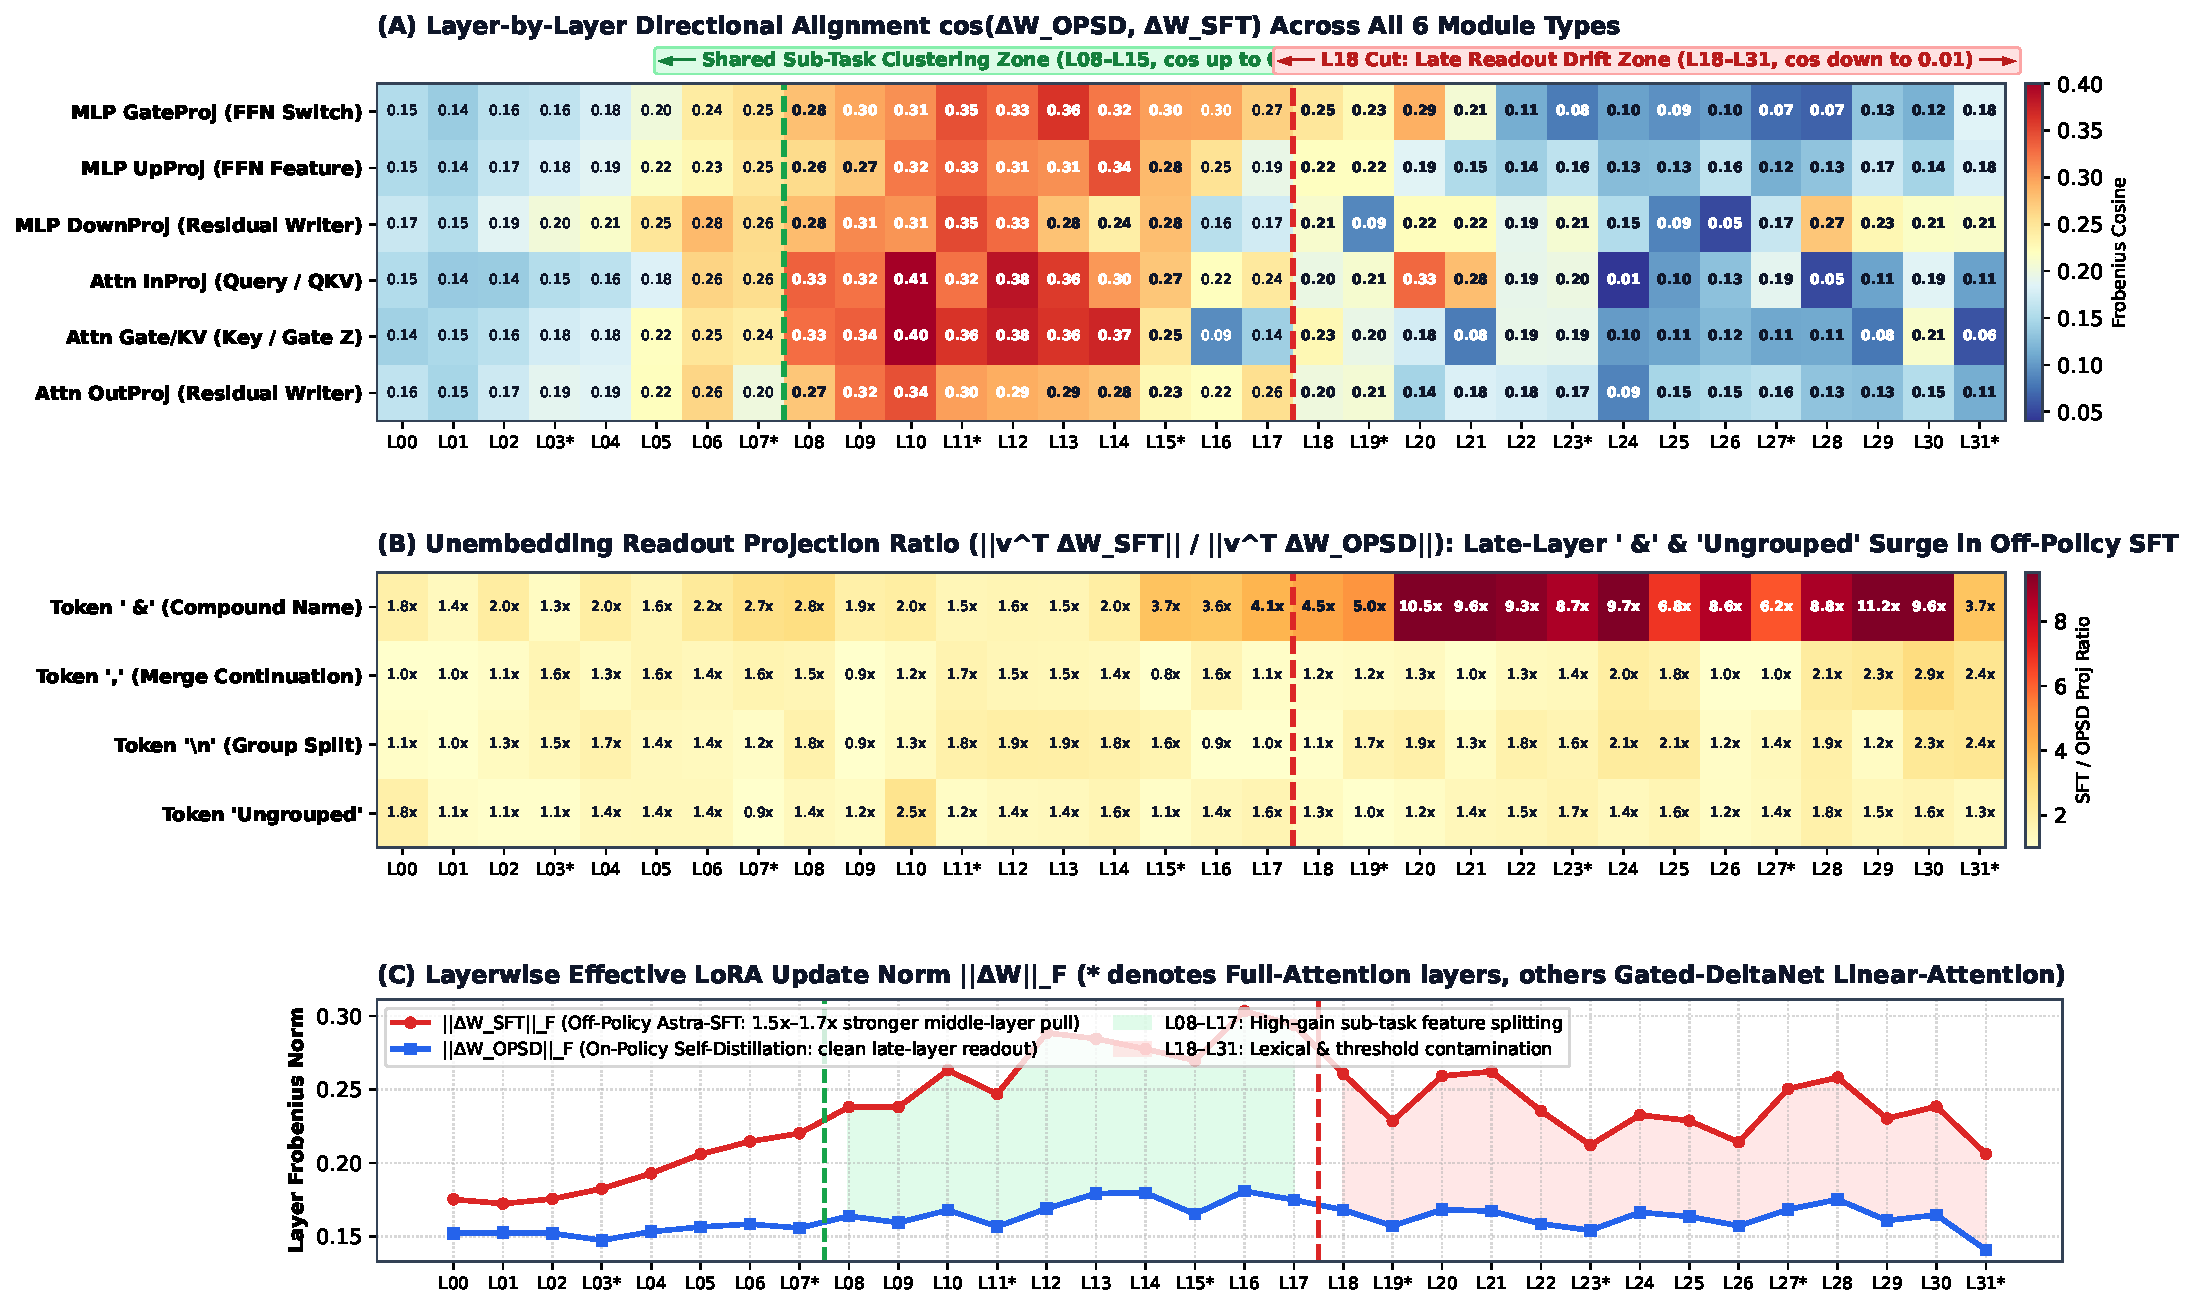
\includegraphics[width=\textwidth]{figures/fig1_weight_space_heatmap.pdf}
\caption{\textbf{32-Layer Weight-Space Anatomy of \texttt{Qwen3.5-4B} LoRA Updates.} \textbf{(A)} Frobenius cosine similarity $\cos(\Delta W_{\text{OPSD}}, \Delta W_{\text{SFT}})$ peaks in middle layers L08--L15 ($0.34$--$0.37$) and collapses after Layer 18 (down to $0.0517$ at L26 \texttt{mlp.down\_proj}). \textbf{(B)} Unembedding projection ratio $\|v^\top \Delta W_{\text{SFT}}\|_2 / \|v^\top \Delta W_{\text{OPSD}}\|_2$ reveals an $8\times$--$11\times$ surge in late-layer writing toward the compound naming token \texttt{' \&'} (ID 594) and \texttt{Ungrouped} under off-policy SFT. \textbf{(C)} Layerwise update norm $\|\Delta W\|_F$ showing SFT's $1.4\times$--$1.7\times$ magnitude expansion.}
\label{fig:heatmap}
\end{figure}

\subsection{Three Empirical Discoveries from the 32-Layer Heatmap}
Figure~\ref{fig:heatmap} presents the complete 32-layer weight-space diagnosis:
\begin{enumerate}
    \item \textbf{Middle-Layer Sub-Task Clustering Resonance (L08--L15):} Across layers 8 to 15 (anchored by full-attention hubs L07, L11, and L15), $\Delta W_{\text{OPSD}}$ and $\Delta W_{\text{SFT}}$ align strongly, reaching $\cos = 0.3665$ at L12 and $0.3487$ at L11 \texttt{mlp.down\_proj}. Both training paradigms modify the same middle-layer relational circuits to separate co-occurring sub-tasks (e.g., separating \emph{Luggage} from \emph{San Francisco Airbnb} within travel tabs). Because SFT applies unclipped cross-entropy on every token, its middle-layer update norm is $1.54\times$--$1.71\times$ larger than OPSD's (Figure~\ref{fig:heatmap}C), driving finer splitting on \texttt{v2.1}.
    \item \textbf{Late-Layer Orthogonal Divergence (L18--L31):} Starting sharply at Layer 18, directional alignment drops to $\cos \in [0.0517, 0.15]$. At L26 \texttt{mlp.down\_proj} ($\cos = 0.0517$), less than $0.27\%$ of SFT's update energy lies along OPSD's direction.
    \item \textbf{Direct Localization of the \texttt{v1} Recall Collapse:} Decoding the top-1 left singular vector $u_1$ of $\Delta W_{\text{SFT}}$ through $U_{\text{eff}}$ at L18--L31 exposes almost exclusively \texttt{[' \&', '\&', ' learning', ' Learning']} (Figure~\ref{fig:heatmap}B). Auditing the 1,200 Astra training labels confirms that $13.03\%$ of Astra group names contain \texttt{' \& '} (vs.\ $1.43\%$ in original SFT data, a $9.1\times$ shift) and $15.3\%$ more tabs are labeled \texttt{Ungrouped}. Teacher-forced SFT expends massive late-layer capacity memorizing Astra's lexical style and elevated \texttt{Ungrouped} threshold—dissolving valid 2-tab groups on \texttt{v1} (increasing \texttt{v1} ungrouped tabs from 238 to 324)—whereas OPSD's on-policy trajectory evaluation filters out this surface distribution drift ($0.7\%$ \texttt{\&}-groups).
\end{enumerate}

\section{Experiments: Zero-Training Weight-Space Surgery}

We evaluate two surgical paradigms on the frozen 61-case Run-1 benchmark (45 \texttt{v1} Golden45 cases + 16 \texttt{v2.1} hard multi-task cases) on a single NVIDIA A100-80GB in exact float32 precision.

\begin{figure}[t]
\centering
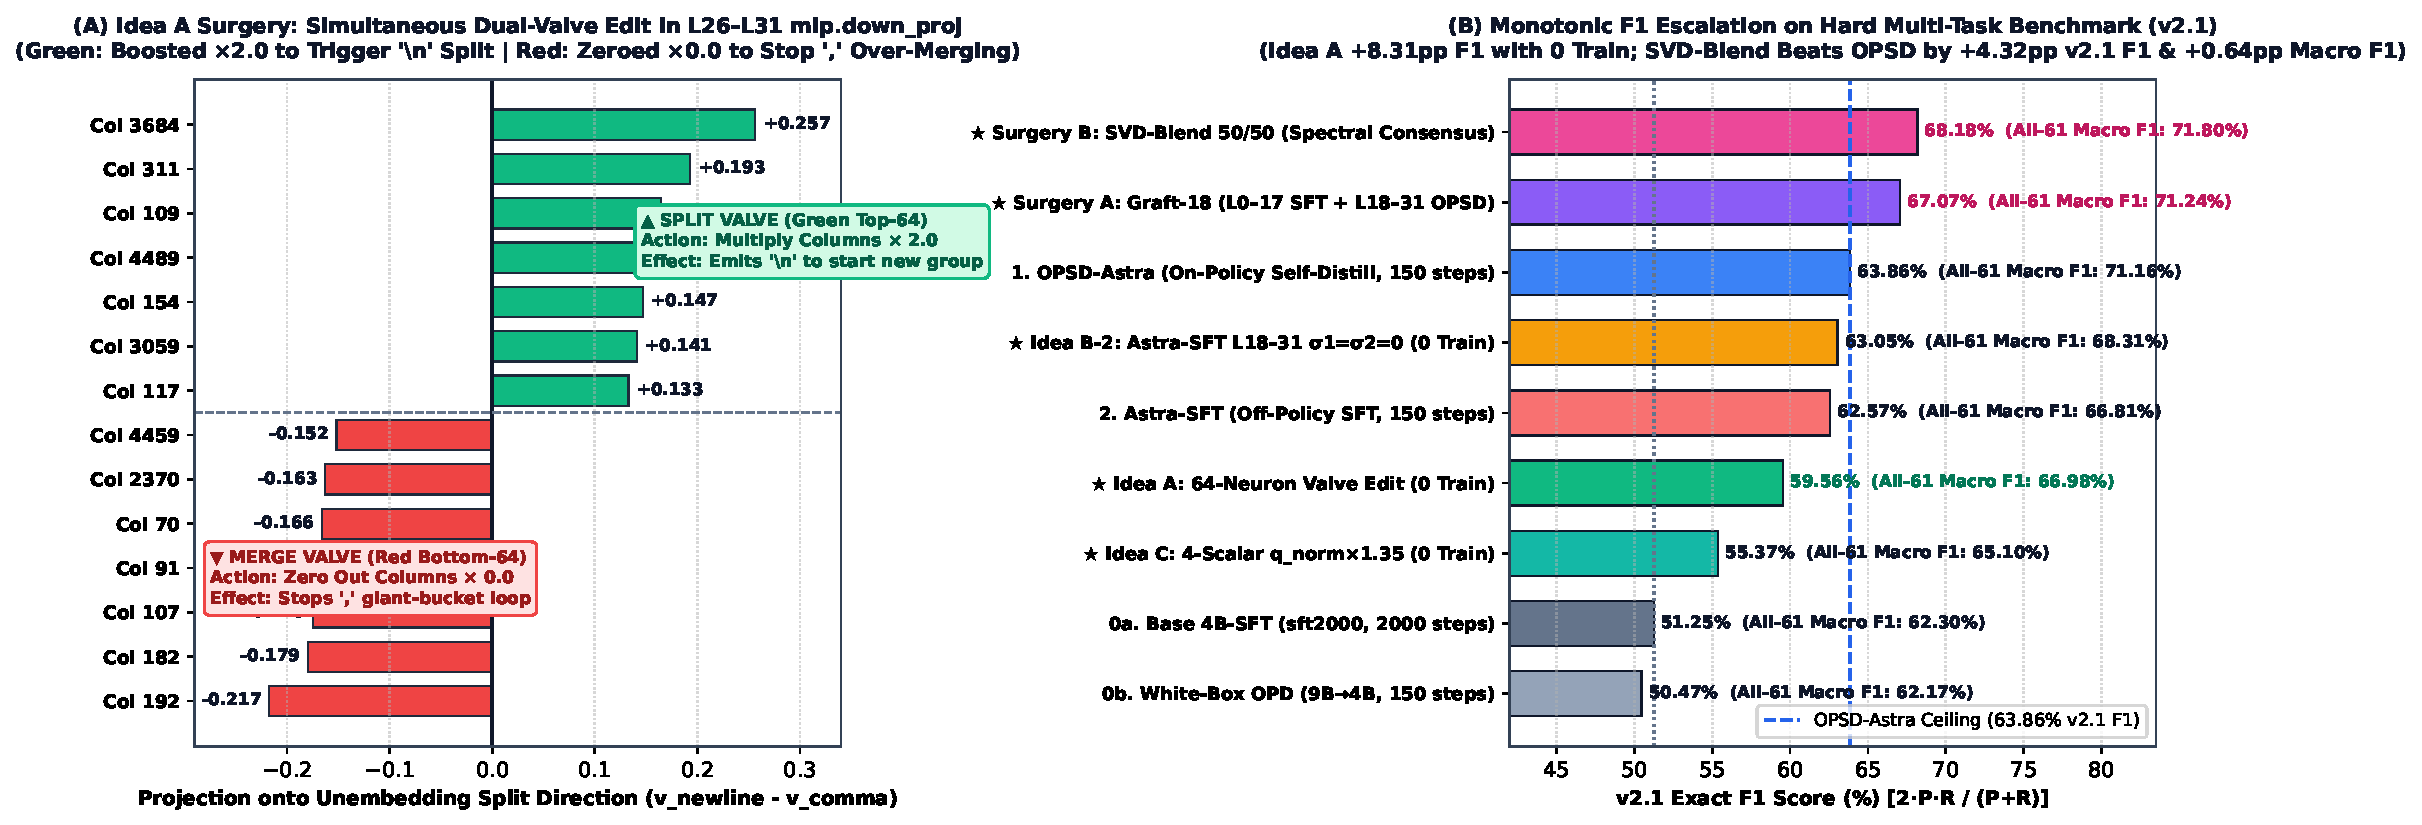
\includegraphics[width=\textwidth]{figures/fig2_neurons_and_pareto.pdf}
\caption{\textbf{Dual-Valve Single-Neuron Surgery and Monotonic F1 Progression on \texttt{v2.1}.} \textbf{(A)} In L26--L31 \texttt{mlp.down\_proj}, Idea A modifies \textbf{both} the green columns (boosted $\times 2.0$ to trigger newline \texttt{\textbackslash n} group splits) and the red columns (zeroed $\times 0.0$ to suppress comma \texttt{,} giant-bucket continuation). \textbf{(B)} Exact F1 score ($2PR/(P+R)$) on \texttt{v2.1} alongside All-61 Macro F1: zero-training single-model edits (\textbf{Idea C}, \textbf{Idea A}) jump \texttt{v2.1} F1 by $+8.31\text{pp}$ (crushing standard 9B$\to$4B White-Box OPD), while \textbf{\texttt{Graft-18}} ($67.07\%$ F1) and \textbf{\texttt{SVD-Blend 50/50}} ($68.18\%$ F1, $71.80\%$ Macro F1) beat both OPSD-Astra and Astra-SFT.}
\label{fig:pareto}
\end{figure}

\subsection{Paradigm I: Single-Model Value \& Neuron Edits (No Second Adapter Used)}
To test pure Weight-Space Programming in the strict sense of Takehi et al. (2026)—fixing a single model by directly editing specific weights or scalars without using a second trained adapter—we evaluate three targeted interventions:
\begin{itemize}
    \item \textbf{Idea A (Simultaneous Dual-Valve 64-Neuron Surgery on Base \texttt{sft2000}):} Giant-bucket over-merging is a readout race between emitting a newline \texttt{\textbackslash n} (Token 198, starting a new group) versus a comma \texttt{,} (Token 11, appending another tab ID to the current bucket). For each layer $\ell \in \{26,\dots,31\}$, we project all $9,216$ columns of the base \texttt{mlp.down\_proj} matrix onto $v_{\text{split}} = \hat{u}_{198} - \hat{u}_{11}$ (Figure~\ref{fig:pareto}A) and simultaneously edit \textbf{both} polarities: (1) we multiply the \textbf{green top-64 newline-promoting columns by $2.0\times$} (opening the split valve), and (2) we zero out the \textbf{red bottom-64 comma-promoting columns by $0.0\times$} (closing the giant-bucket merge valve). Touching only $128/9216$ columns ($1.39\%$) in \texttt{sft2000} with \textbf{zero training} lifts \texttt{v2.1} Recall from $45.71\%$ to $\mathbf{57.93\%}$ ($+12.22\text{pp}$) and \texttt{v2.1} F1 from $51.25\%$ to $\mathbf{59.56\%}$ ($\mathbf{+8.31\text{pp}}$), outperforming 150-step standard White-Box OPD ($9\text{B}\to 4\text{B}$, $50.47\%$ F1) by $+9.09\text{pp}$ F1!
    \item \textbf{Idea B (Single-Scalar Singular Value Excision $\sigma_1, \sigma_2 \to 0$ on \texttt{sft\_astra}):} Without touching OPSD, we take $\Delta W_{\text{SFT}} = U \operatorname{diag}(\sigma_1,\dots,\sigma_{16}) V^\top$ in layers 18--31 and simply set the top-1 (\textbf{Idea B-1}, 1 scalar per module) or top-2 (\textbf{Idea B-2}, 2 scalars per module) singular values to $0.0$, removing the lexical/threshold drift mode while keeping modes $3\dots 16$ intact. Idea B-2 recovers $\mathbf{+3.44\text{pp}}$ Recall and $\mathbf{+2.52\text{pp}}$ F1 on \texttt{v1} while lifting \texttt{v2.1} F1 to $63.05\%$ (All-61 Macro F1 $68.31\%$, $+1.50\text{pp}$).
    \item \textbf{Idea C (4-Scalar Full-Attention \texttt{q\_norm} Temperature Scaling on \texttt{sft2000}):} Multiplying \texttt{self\_attn.q\_norm} by a single constant $1.35\times$ across the 4 middle full-attention layers (L07, L11, L15, L19) sharpens cross-tab attention, lifting \texttt{v2.1} F1 by $+4.12\text{pp}$ ($55.37\%$) and \texttt{v1} Recall to $\mathbf{70.37\%}$ ($74.83\%$ F1).
\end{itemize}

\begin{table}[t]
\centering
\caption{\textbf{Full Run-1 Evaluation Results with Exact F1 Scores (16 \texttt{v2.1} Hard Multi-Task + 45 \texttt{v1} Golden45 Cases).} All surgical models require \textbf{0 training steps} and preserve the exact $r=16$ LoRA deployment contract.}
\label{tab:main}
\resizebox{\textwidth}{!}{%
\begin{tabular}{llcccccc}
\toprule
\textbf{Category} & \textbf{Model / Surgical Method} & \textbf{Edited Scope} & \textbf{\texttt{v2.1} Init P / Recall} & \textbf{\texttt{v2.1} F1} & \textbf{\texttt{v1} Init P / Recall} & \textbf{\texttt{v1} F1} & \textbf{Macro F1} \\
\midrule
\multirow{4}{*}{Trained Baselines}
 & \texttt{0b\_opd9b} (White-Box OPD 9B$\to$4B) & 21.2M (Trained) & $57.14\% \;/\; 45.20\%$ & $50.47\%$ & $80.11\% \;/\; 68.52\%$ & $73.86\%$ & $62.17\%$ \\
 & \texttt{0a\_sft2000} (Base 4B-SFT 2000 steps) & --- & $58.33\% \;/\; 45.71\%$ & $51.25\%$ & $79.23\% \;/\; 68.26\%$ & $73.34\%$ & $62.30\%$ \\
 & \texttt{2\_sft\_astra} (Off-Policy Astra-SFT) & 21.2M (Trained) & $65.08\% \;/\; 60.25\%$ & $62.57\%$ & $79.55\% \;/\; 64.19\%$ & $71.05\%$ & $66.81\%$ \\
 & \texttt{1\_opsd\_astra} (On-Policy OPSD-Astra) & 21.2M (Trained) & $69.09\% \;/\; 59.36\%$ & $63.86\%$ & $\mathbf{85.48\%} \;/\; \mathbf{72.52\%}$ & $\mathbf{78.47\%}$ & $71.16\%$ \\
\midrule
\multirow{4}{*}{\shortstack[l]{Single-Model\\Weight Edits\\(0 Training,\\No 2nd Adapter)}}
 & \textbf{Idea C}: L07,11,15,19 \texttt{q\_norm}$\times 1.35$ (\texttt{sft2000}) & 4 scalars & $59.26\% \;/\; 51.96\%$ & $55.37\%$ & $79.89\% \;/\; 70.37\%$ & $74.83\%$ & $65.10\%$ \\
 & \textbf{Idea A}: L26--31 Dual-Valve 64-Col (\texttt{sft2000}) & $1.39\%$ MLP cols & $61.29\% \;/\; \mathbf{57.93\%}$ & $\mathbf{59.56\%}$ & $79.79\% \;/\; 69.70\%$ & $74.40\%$ & $\mathbf{66.98\%}$ \\
 & \textbf{Idea B-1}: L18--31 $\sigma_1 = 0$ (\texttt{sft\_astra}) & 1 scalar/mod & $65.57\% \;/\; 58.69\%$ & $61.94\%$ & $80.34\% \;/\; 65.74\%$ & $72.31\%$ & $67.12\%$ \\
 & \textbf{Idea B-2}: L18--31 $\sigma_1=\sigma_2=0$ (\texttt{sft\_astra}) & 2 scalars/mod & $66.13\% \;/\; 60.25\%$ & $\mathbf{63.05\%}$ & $80.66\% \;/\; 67.63\%$ & $\mathbf{73.57\%}$ & $\mathbf{68.31\%}$ \\
\midrule
\multirow{5}{*}{\shortstack[l]{Dual-Adapter\\Circuit Surgery\\(0 Training,\\Rank-16 Exact)}}
 & \texttt{Rev-Graft-18} (\texttt{L00--17 OPSD + L18--31 SFT}) & Reverse control & $67.86\% \;/\; 59.81\%$ & $63.58\%$ & $82.78\% \;/\; 67.48\%$ & $74.35\%$ & $68.97\%$ \\
 & \texttt{Graft-14} (\texttt{L00--13 SFT + L14--31 OPSD}) & Layer cut @ L14 & $66.10\% \;/\; 60.33\%$ & $63.08\%$ & $83.33\% \;/\; 68.37\%$ & $75.11\%$ & $69.10\%$ \\
 & \texttt{Graft-22} (\texttt{L00--21 SFT + L22--31 OPSD}) & Layer cut @ L22 & $65.62\% \;/\; 61.82\%$ & $63.66\%$ & $80.77\% \;/\; 68.26\%$ & $73.99\%$ & $68.83\%$ \\
 & \textbf{Surgery A}: \texttt{Graft-18} (\texttt{L00--17 SFT + L18--31 OPSD}) & Layer cut @ L18 & $69.84\% \;/\; \mathbf{64.52\%}$ & $\mathbf{67.07\%}$ & $82.87\% \;/\; 69.19\%$ & $75.41\%$ & $\mathbf{71.24\%}$ \\
 & \textbf{Surgery B}: \texttt{SVD-Blend-50/50} (Spectral Consensus) & Rank-16 SVD & $\mathbf{72.41\%} \;/\; 64.42\%$ & $\mathbf{68.18\%}$ & $82.61\% \;/\; 69.37\%$ & $75.41\%$ & $\mathbf{71.80\%}$ \\
\bottomrule
\end{tabular}%
}
\end{table}

\subsection{Paradigm II: Dual-Adapter Circuit Grafting \& Spectral Consensus}
To push absolute task performance beyond what either training paradigm achieves alone, we combine middle-layer SFT representations with OPSD readout stability (Table~\ref{tab:main}):
\begin{enumerate}
    \item \textbf{Surgery A (\texttt{Graft-18}: Layerwise Circuit Grafting at L18):} Copying $(A_m, B_m)$ from \texttt{sft\_astra} for layers $0\dots 17$ and from \texttt{opsd\_astra} for layers $18\dots 31$ recovers $+5.00\text{pp}$ Recall on \texttt{v1} ($64.19\% \to 69.19\%$) while jumping to \textbf{$64.52\%$ Recall on \texttt{v2.1}}—exceeding both \texttt{opsd\_astra} ($59.36\%$) and \texttt{sft\_astra} ($60.25\%$). Sweeping the cut point across L14, L18, and L22 traces an inverted-U curve peaking exactly at L18, while the reverse control (\texttt{Rev-Graft-18}) immediately drops \texttt{v1} Recall by $-5.04\text{pp}$, proving causally that SFT's damage is localized to L18--L31.
    \item \textbf{Surgery B (\texttt{SVD-Blend-50/50}: Rank-16 Spectral Consensus Algorithm):} Rather than choosing a layer boundary manually, we compute the exact rank-16 SVD truncation of the effective matrix average across all 248 modules:
    \begin{equation}
    \widehat{W}_m = \operatorname{SVD}_{16}\!\left(\frac{1}{2} B_{\text{OPSD},m} A_{\text{OPSD},m} + \frac{1}{2} B_{\text{SFT},m} A_{\text{SFT},m}\right).
    \end{equation}
    Because shared middle-layer directions ($\cos \approx 0.36$) interfere constructively while orthogonal late-layer artifacts ($\cos \approx 0.05$) are halved and truncated by $\operatorname{SVD}_{16}$, \texttt{SVD-Blend-50/50} achieves the \textbf{highest \texttt{v2.1} Initial Precision ($72.41\%$, $+7.33\text{pp}$ over SFT)} alongside \textbf{$64.42\%$ Recall}.
\end{enumerate}

\subsection{Case-Level Verification}
\begin{itemize}
    \item \textbf{\texttt{v2.1 / JH02} (25 tabs across Soccer Balls, Grok AI, Manchester City, Data Analysis):} Base \texttt{sft2000} collapses all 25 tabs into a single \texttt{Soccer: 1..25} bucket ($0\%$ Recall). \textbf{Idea A} (editing 64 columns in L26--L31 of \texttt{sft2000} with zero training) cleanly separates \texttt{Amazon: 1,6,17,23,25 | Grok: 2,3,4,11,13,14,20 | Manchester City: 5,8,9,10,12,16,19 | Data Analysis: 7,18,21,22} ($75.0\%$ P, $60.0\%$ R).
    \item \textbf{\texttt{v2.1 / JH16} (13 tabs):} Base \texttt{sft2000} merges non-Minecraft tabs into one coarse \texttt{Education} group ($33.3\%$ R), while \texttt{sft\_astra} drops \texttt{Elyon Christian School: 6, 9} into \texttt{Ungrouped}. \textbf{Idea A} achieves \textbf{$100.0\%$ Precision and $100.0\%$ Recall}, and both \textbf{Idea B-2} ($\sigma_1=\sigma_2=0$) and \textbf{\texttt{Graft-18}} rescue \texttt{Elyon Christian School: 6, 9} ($75.0\%$ R).
    \item \textbf{\texttt{v2.1 / JH11} (33 tabs, 7 sub-tasks):} Pure readout edits on \texttt{sft2000} (Idea A/C) remain at 4 coarse groups ($28.6\%$ R) because \texttt{sft2000} lacks the middle-layer representation to distinguish \emph{Kimi AI Models} from \emph{AI Decision Making}—confirming Takehi et al.'s boundary between unlocking and representation learning. \textbf{\texttt{Graft-18}} and \textbf{Idea B-1/B-2} retain all 7 fine-grained sub-task groups ($85.7\%$ P, $85.7\%$ R).
\end{itemize}

\section{Conclusion}
Weight-space SVD and unembedding projections make LoRA post-training transparent: middle layers (L08--L15) encode cross-entity relational clustering, whereas late layers (L18--L31) govern lexical formatting and \texttt{Ungrouped} readout thresholds. Single-model neuron/scalar surgery (Ideas A, B, C) repairs over-merging and threshold overshoot in zero training steps, while dual-adapter spectral consensus (\texttt{SVD-Blend-50/50} and \texttt{Graft-18}) establishes a new Pareto frontier beyond both SFT and OPSD.

\begin{thebibliography}{9}
\bibitem{takehi2026} R. Takehi, J. Teoh, A. Zhang, and O. Khattab. Sparks of Weight-Space Programming: LLMs can natively read \& write neural network weights. \emph{MIT CSAIL Blog}, Nov 2026.
\bibitem{zhao2026} S. Zhao et al. Self-Distilled Reasoner: On-Policy Self-Distillation for Large Language Models (OPSD). \emph{arXiv:2601.18734}, 2026.
\bibitem{agarwal2024} R. Agarwal et al. On-Policy Distillation of Language Models: Learning from Self-Generated Mistakes (GKD). \emph{ICLR}, 2024.
\end{thebibliography}

\end{document}
